% D3RA-DNA manuscript (revision 3: computational-only positioning, digital-twin primary evidence,
% leak-free secondary replay).  Official IEEEtran class (v1.8b, CTAN), following bare_conf.tex.
\documentclass[conference]{IEEEtran}
\IEEEoverridecommandlockouts
\usepackage{cite}
\usepackage{amsmath,amssymb,amsfonts}
\usepackage{graphicx}
\usepackage{textcomp}
\usepackage{url}
\usepackage{xcolor}
\usepackage{booktabs}
\usepackage{multirow}
\usepackage{array}
\usepackage{tikz}
\usetikzlibrary{arrows.meta,positioning,fit,shapes.geometric,calc}
\newcommand{\E}{\mathbb{E}}
\newcommand{\Prob}{\mathbb{P}}
\graphicspath{{figures/}}
\input{tables/macros}

\begin{document}

\title{Verified Stopping, Not Adaptive Allocation, Saves Reads in Multi-Container DNA Storage: A Leak-Free Computational Study on a Digital Twin and Real Read Streams}

\author{\IEEEauthorblockN{Sai Mouli}
\IEEEauthorblockA{saimouli12345678@gmail.com}
}

\maketitle

\begin{abstract}
When an erasure-coded DNA archive is spread over several separately synthesised and handled
containers of unknown quality, two retrieval decisions arise: when to stop sequencing and which
container to read next.  We find that the first matters and the second, as usually modelled, does
not.  All work is computational; nothing was synthesised or sequenced.  On the DT4DDS digital twin
with six independently synthesised, aged and amplified containers, a streaming decoder that stops
only when every stripe, its CRC-32 and the file's SHA-256 verify used on average 27\% fewer reads
than the best hindsight-tuned static plan must reserve (3.49k vs.\ 4.80k), with no model at all.
Model-based container selection, including Thompson sampling, UCB, learn-then-commit and
information-greedy rules, was a measured negative when one container was near-dead ($+$7\% to
$+$441\% reads against round-robin), because one efficiency multiplier cannot represent dropout; it
helped only after an outright container failure (up to $-$24\%) or under mild heterogeneity
($-$2 to $-$4\%).  No rule lowered the 0.99-quantile.  Over \SafeN{} end-to-end retrievals with no
oracle, no output file was wrong (exact 95\% upper limit \SafeWUB{}) and no wrong payload passed the inner
checks in \SafeAtt{} decodes (bound \SafeFUB{}).  A leak-free replay of real Illumina read streams
from two vendors (secondary, oracle decodability) agrees: stopping cut reads against fixed depth by
14\% and 25\%, and allocation with a generic prior changed them by at most 3\%; only a prior
calibrated on held-out reads of the same containers, which identified a near-dead container in
advance, saved more (16\% on one pool).
Every number is regenerated from committed result files under a frozen protocol with logged
deviations, and sampled retrievals re-run bit for bit.
\end{abstract}

\begin{IEEEkeywords}
DNA data storage, adaptive sequencing, verified stopping, erasure coding, coverage depth, digital twin, Bayesian calibration, multi-armed bandits, reproducibility
\end{IEEEkeywords}

%=====================================================================
\section{Introduction}
%=====================================================================
DNA has been demonstrated as an archival medium at kilobyte to hundreds-of-megabyte
scale~\cite{church2012next,goldman2013towards,grass2015robust,erlich2017fountain,organick2018random}.
Retrieval requires sequencing, which samples molecules at random: some strands are read
many times, others never, and reads carry substitution, insertion and deletion
errors~\cite{heckel2019characterization,gimpel2023digital}.  Systems therefore protect each
strand with an inner code and groups of strands with an outer erasure code, and sequence to a
fixed depth expected to recover enough strands~\cite{grass2015robust,organick2018random}.  The
number of reads needed for decoding---the \emph{coverage depth}---is now studied in its own
right~\cite{barlev2025cover,gruica2024combinatorial}.

We consider archives split across several physically separate \emph{containers} (vials,
capsules, pools) that are synthesised, stored and handled separately.  This is a working
assumption rather than established practice; random access so far addresses files within one
pool~\cite{bornholt2016dna,organick2018random}, and recent theory treats erasure-coded data
partitioned over containers with uniform sampling~\cite{kong2026coverage} and container
failures~\cite{levy2026expected}.  Containers age, are amplified and fail differently, and
these differences are unknown when a retrieval starts.  Two operational questions follow:
\emph{when} to stop sequencing, and \emph{which} container to sequence next.

\textbf{Problem.}  Given an erasure-coded file distributed over $M$ containers of unknown,
heterogeneous quality, some of which may have failed, sequence in batches and decide after
each batch which container to read and whether to stop, so that the output file is
byte-identical to the stored one with high probability while the number of reads is small.

\textbf{Findings.}  (i) \emph{Verified stopping is the robust saving}: it needs no model, never
returned a wrong file, and lowered the mean reads per retrieval against fixed-depth sequencing in
every setting (digital twin and both real-read pools) and against the hindsight-tuned static plan
on the digital twin and the Twist replay; on the Genscript replay the hindsight plan, which knows
in advance to avoid a near-dead container, was 1\% cheaper.  (ii) \emph{Adaptive allocation is a measured negative} when
a container is near-dead: every model-based rule we tried read more than round-robin; it helps only
after an outright failure, under mild heterogeneity, or when calibration data identify the weak
container before retrieval.  (iii) No rule lowers the 0.99-quantile, so
the gains serve pay-per-read users, not users who reserve capacity.  (iv) Two results mark the
\emph{design boundaries} of the archive rather than of the policies: with two failed containers or
with a noisier (photolithographic) synthesis model, the file is unrecoverable by any policy.

\textbf{Scope.}  All work is computational.  Nothing was synthesised or sequenced for this
paper, and no result should be read as a wet-lab demonstration.  We use the term \emph{exact
retrieval} only for our digital-twin pipeline, where the output file is checked byte for byte
against the stored file; on replayed real reads, decodability is an oracle event and we speak
of \emph{recovery}.

\textbf{Contributions.}
\begin{enumerate}
\item \emph{Evidence that verified stopping is the robust saving.}  A verification-gated streaming
retrieval pipeline that stops only when every stripe, its CRC-32 and the file's SHA-256 verify
(Section~\ref{sec:method}), evaluated against a static family that includes a hindsight-tuned plan.
Stopping when decodable~\cite{lopez2019dna} and checksum-verified decoding~\cite{erlich2017fountain}
are known; quantifying their value for multi-container retrieval is, to our knowledge, new.
\item \emph{A measured negative for adaptive allocation.}  An online-adaptive controller family (a
discrete posterior over container efficiency with a failure atom and a beta-binomial likelihood,
and eight rules including Thompson sampling, UCB, learn-then-commit and information-greedy
design~\cite{thompson1933likelihood,auer2002finite,garivier2016explore,chaloner1995bayesian})
loses to round-robin under a near-dead container; we identify the cause (a single efficiency
multiplier cannot represent dropout), map where allocation helps (outright failure, mild
heterogeneity) with a severity sweep, and show that the better-calibrated likelihood allocates
worse.
\item \emph{Leak-free, end-to-end reproducibility and safety bounds.}  The full chain from DT4DDS
reads~\cite{gimpel2023digital} of independently synthesised containers to bytes, with no oracle,
under a protocol frozen before the final runs; exact bounds on wrong outputs and false accepts; a
leak-free re-analysis of real Illumina streams, with our earlier leaky analysis kept as an upper
bound (Appendix~\ref{app:leak}); bit-for-bit re-runs and a claim-to-evidence map
(Section~\ref{sec:repro}).
\end{enumerate}

%=====================================================================
\section{Background and Related Work}\label{sec:related}
%=====================================================================
\textbf{DNA storage systems and channels.}  Storage systems combine constrained encodings with
inner and outer codes~\cite{antkowiak2020low,goldman2013towards,grass2015robust,erlich2017fountain,organick2018random,press2020hedges}.
Coverage is over-dispersed, a few percent of strands drop out, and errors arise mostly in
synthesis and sequencing~\cite{heckel2019characterization,chen2020quantifying,gimpel2023digital}.
DT4DDS~\cite{gimpel2023digital} is a digital twin of the synthesis, aging, PCR and sequencing
steps whose error and bias parameters were fitted to experiments; we use it as the simulator of
our primary evidence.  Information-theoretic models treat the channel as sampling with
replacement followed by noise~\cite{shomorony2021dna,weinberger2022dna,lenz2020coding}.

\textbf{Coverage depth.}  For a sampler that cannot be controlled, MDS codes and uniform
sampling minimise the expected number of reads~\cite{barlev2025cover}.  Follow-ups study random
access~\cite{gruica2024combinatorial}, real-data sampling distributions~\cite{cao2025optimizing},
partitioning over containers~\cite{kong2026coverage}, container failures~\cite{levy2026expected}
and the reliability of MDS-coded retrieval~\cite{kashanna2026reliability}.  These works analyse
\emph{fixed} sampling laws; we study a \emph{controllable} sampler.

\textbf{Adaptive sequencing and sequential decisions.}  Nanopore adaptive sampling selects
molecules in real time~\cite{loose2016real,payne2021readfish,weilguny2023dynamic}, and
DNA-storage readouts have been sequenced until sufficient coverage~\cite{lopez2019dna}.
Choosing a container resembles a multi-armed bandit with a combinatorial ($K$-of-$N$ per stripe)
reward; we use Thompson sampling~\cite{thompson1933likelihood,russo2018tutorial}, upper
confidence bounds~\cite{auer2002finite}, explore-then-commit~\cite{garivier2016explore} and an
information-greedy rule from Bayesian experimental design~\cite{chaloner1995bayesian} as
baselines (see~\cite{lattimore2020bandit}).  We prove no regret bound.

\textbf{Placement and consensus.}  Erasure-coded storage limits the fragments of a stripe per
failure domain~\cite{weil2006crush,cidon2013copysets,ford2010availability,nath2006subtleties,leong2012distributed}.
Strands are reconstructed from noisy reads by trace
reconstruction~\cite{batu2004reconstructing,srinivasavaradhan2021trellis,sabary2024reconstruction}
after clustering~\cite{rashtchian2017clustering} or learned models~\cite{barlev2025deep};
systematic nanopore errors are documented~\cite{delahaye2021sequencing,wick2019performance}.
Table~\ref{tab:literature_comparison} positions this work.
\input{tables/literature_comparison}

%=====================================================================
\section{System Model}\label{sec:model}
%=====================================================================
\begin{figure*}[t]
\centering
\resizebox{\textwidth}{!}{%
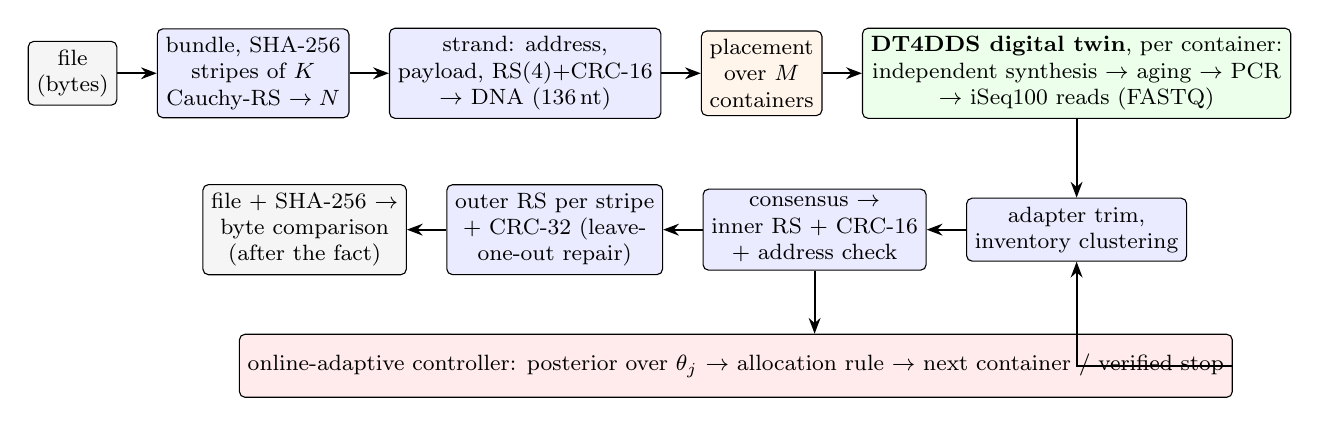
\begin{tikzpicture}[font=\footnotesize, node distance=4mm and 5mm,
  box/.style={draw, rounded corners=2pt, align=center, minimum height=8mm, inner sep=3pt, fill=#1!8},
  box/.default=blue, arr/.style={-{Stealth[length=2mm]}, thick}]
\node[box=gray] (files) {file\\(bytes)};
\node[box, right=of files] (stripes) {bundle, SHA-256\\stripes of $K$\\Cauchy-RS $\to N$};
\node[box, right=of stripes] (strands) {strand: address,\\payload, RS(4)+CRC-16\\$\to$ DNA (136\,nt)};
\node[box=orange, right=of strands] (place) {placement\\over $M$\\containers};
\node[box=green, right=of place, minimum width=36mm] (dt) {\textbf{DT4DDS digital twin}, per container:\\independent synthesis $\to$ aging $\to$ PCR\\$\to$ iSeq100 reads (FASTQ)};
\node[box, below=10mm of dt] (clus) {adapter trim,\\inventory clustering};
\node[box, left=of clus] (cons) {consensus $\to$\\inner RS + CRC-16\\+ address check};
\node[box, left=of cons] (outer) {outer RS per stripe\\+ CRC-32 (leave-\\one-out repair)};
\node[box=gray, left=of outer] (out) {file + SHA-256 $\to$\\byte comparison\\(after the fact)};
\node[box=red, below=8mm of cons, minimum width=110mm, xshift=-10mm] (ctl) {online-adaptive controller: posterior over $\theta_j$ $\to$ allocation rule $\to$ next container / verified stop};
\draw[arr] (files)--(stripes); \draw[arr] (stripes)--(strands); \draw[arr] (strands)--(place); \draw[arr] (place)--(dt);
\draw[arr] (dt)--(clus); \draw[arr] (clus)--(cons); \draw[arr] (cons)--(outer); \draw[arr] (outer)--(out);
\draw[arr] (cons.south) -- (cons.south |- ctl.north); \draw[arr] (ctl.east) -| (clus.south);
\end{tikzpicture}}
\caption{Pipeline of the primary experiments (conceptual diagram).  Every container is an
independent DT4DDS synthesis with its own handling history; its reads are consumed in batches
by the same streaming decoder that reads FASTQ files.  The true file is used only after a
retrieval ends, to count wrong outputs and false accepts.}
\label{fig:arch}
\end{figure*}

Table~\ref{tab:notation} lists the notation.
\input{tables/notation}

\subsection{Storage}
A file is bundled, hashed (SHA-256) and split into $S$ stripes of $K$ data fragments of $P$
bytes.  A systematic Cauchy Reed--Solomon code~\cite{reed1960polynomial} over GF($2^8$) extends
each stripe to $N$ fragments, any $K$ of which suffice.  Each fragment becomes a strand carrying
an address, an address check byte, the payload and an inner Reed--Solomon code with four parity
bytes plus a CRC-16, mapped to DNA by a whitened 2-bit code.  Code parameters, a CRC-32 per
stripe and the SHA-256 are kept in a manifest outside the DNA.  Fragments are assigned
round-robin to $M$ containers.

\subsection{Sequencing and recovery model used by the controller}
Reads from container $j$ form a stream.  The controller's model (used only to rank containers
and to forecast; never to decide that a fragment is recovered) treats the reads of a stored
fragment as negative-binomial with mean $\theta_j\,R_j\,\bar\pi_j$ after $R_j$ reads, where
$\bar\pi_j$ is the prior per-fragment read share (yield over stored fragments) and $\theta_j$ an
unknown efficiency multiplier ($\theta_j{=}0$: failed container).  A fragment becomes decodable
after $t$ reads with probability $\varphi(t)$ (consensus-success curve), and a molecule is absent
with probability $d$ (dropout).  Integrating over abundance gives the probability $Q(\mu)$ that a
stored fragment is decodable at mean coverage $\mu$:
\begin{equation}
Q(\mu)=(1-d)\,\E_g\Big[\sum_{n\ge0}\mathrm{NB}(n;k,g\mu)\,\varphi(n)\Big],
\label{eq:Q}
\end{equation}
with a shared log-normal strand effect $g$ (Gauss--Hermite quadrature).  Every container starts
from the same generic literature prior (yield 0.9, NB shape $k{=}10$, dropout 0.5\%, a generic
consensus curve, failure probability $10^{-3}$); no calibration data of the evaluated system is
used in the primary experiments.

\subsection{Objective and who benefits}
A policy chooses, after each batch of $b$ reads, a container and whether to stop.  We report two
costs because they serve different users.  A \emph{pay-per-read} user (e.g.\ streaming nanopore
sequencing, or a service that bills reads) pays the reads actually used: the relevant metric is
the \emph{mean} reads per retrieval.  A user who must \emph{reserve} capacity in advance (e.g.\ a
fixed flowcell) pays for the 0.99-quantile (q99) on every retrieval.  A static plan, which
commits read proportions and a budget in advance, pays its q99 every time; its mean cost
\emph{is} its q99.  Adaptive stopping helps the first user even when it does not reduce q99.

%=====================================================================
\section{Online-Adaptive Retrieval}\label{sec:method}
%=====================================================================
\subsection{Posterior over container efficiency}
The support of $\theta_j$ is $\Theta=\{0\}\cup\{\theta^{(1)},\dots,\theta^{(25)}\}$, log-spaced in
$[0.01,5]$, with prior $p_0(0)=f_j$ and $p_0(\theta^{(\ell)})\propto(1-f_j)\exp(-\frac12(\ln\theta^{(\ell)}/s)^2)$,
with $s=0.5$ in every policy run.  After $R_j$ reads with $U_j$ verified fragments among the $n_j$ stored in container
$j$, we use a beta-binomial likelihood with intra-container correlation $\rho_U$:
\begin{equation}
p(\theta\mid R_j,U_j)\propto p_0(\theta)\,\mathrm{BB}\big(U_j;\,n_j,\,Q(\theta R_j\bar\pi_j),\,\rho_U\big),
\label{eq:posterior}
\end{equation}
where $\mathrm{BB}(u;n,p,\rho)$ has mean $np$ and variance $np(1-p)(1+(n-1)\rho)$; $\rho_U{=}0$
recovers the binomial.  Recoveries of a container's fragments are correlated (shared synthesis
bias, dropout), so the binomial is over-confident; $\rho_U$ is chosen on disjoint calibration
replicates (Section~\ref{sec:calib-protocol}).  We call the controller \emph{online-adaptive},
not self-calibrating: it adapts to observations, but its uncertainty is not well calibrated
(Section~\ref{sec:res-calib}).

\subsection{Allocation rules}
For an unrecovered fragment $i$ in container $j$, the hazard of becoming decodable within the
next $b$ reads is
$h_{ij}=[Q(\tilde\theta_j(R_j{+}b)\bar\pi_j)-Q(\tilde\theta_jR_j\bar\pi_j)]/[1-Q(\tilde\theta_jR_j\bar\pi_j)]$,
where $\tilde\theta_j$ is chosen by the rule:
\begin{itemize}
\item \emph{Round-robin + verified stop}: reads every container in turn (no model).
\item \emph{Coverage-greedy}: $\tilde\theta_j$ = posterior mean; reads $\arg\max_j\sum_i h_{ij}$
over fragments of unfinished stripes.
\item \emph{Pivotal}: weights each fragment by a normal-approximation sensitivity of its
stripe's completion probability (our earlier rule; details in the supplement).
\item \emph{Thompson sampling}~\cite{thompson1933likelihood,russo2018tutorial}: $\tilde\theta_j$
drawn from the posterior; coverage score.
\item \emph{UCB}~\cite{auer2002finite}: $\tilde\theta_j$ = posterior 0.9-quantile.
\item \emph{Learn-then-commit}~\cite{garivier2016explore}: five round-robin batches per
container, then the posterior is frozen and the coverage score used.
\item \emph{Info-greedy} (Bayesian experimental design~\cite{chaloner1995bayesian}): reads the
container with the largest posterior variance of $\ln\theta_j$ until all fall below $10^{-3}$,
then coverage-greedy.
\item \emph{Tail-aware}: $\tilde\theta_j$ = posterior 0.1-quantile (pessimistic) and the score
counts only the 10\% of stripes with the largest remaining need (the bottleneck stripes that
set the retrieval's length); a heuristic aimed at the q99.
\end{itemize}
All rules probe each container with one batch first.  The \emph{static} family reads fixed
proportions $w_j\propto e_j^{\alpha}$, $\alpha\in\{0,0.5,1,2\}$, until decodable, where $e_j$ is
the per-read recovery rate of container $j$ measured in hindsight on the same scenario:
$\alpha{=}0$ is uniform fixed depth, $\alpha{=}1$ equalises expected coverage, and the best
$\alpha$ is a hindsight-tuned (``oracle'') static plan.

\subsection{Verified stopping}
A retrieval stops with an output file only when (i) every stripe holds $K$ fragments that each
passed inner RS decoding, CRC-16 and the address check, (ii) every stripe matches its CRC-32, and
(iii) the file matches its SHA-256.  If (ii) fails, one more fragment is requested for that
stripe and the faulty fragment is localised by leave-one-out decoding.  If the streams are
exhausted first, the retrieval reports failure; it never returns an unverified file.  An
early-abandonment (futility) rule is disabled in all runs.

\subsection{Completion forecast}
The controller also forecasts the probability of finishing within a remaining budget.  The
\emph{analytic} forecast multiplies per-stripe normal approximations of
$\Prob(\sum_{i\in s}X_i\ge\nu_s)$ with the remaining budget spread evenly over containers.  The
\emph{posterior-simulation} forecast (default) draws 200 values of $\theta$ from the posterior,
spreads the remaining budget in proportion to the reads spent so far, simulates per-fragment
recoveries and reports the fraction of draws in which every stripe completes.

%=====================================================================
\section{Evaluation Methodology}\label{sec:eval}
%=====================================================================
\subsection{Digital-twin end-to-end pipeline (primary evidence)}
We store a fixed 18{,}432-byte random file with $P{=}24$-byte payloads, $(K,N)=(32,48)$, 25
stripes and 1{,}200 strands of 136\,nt over $M{=}6$ containers.  For each container we run
DT4DDS~1.1.0~\cite{gimpel2023digital} with its published default parameters: array synthesis
(Twist model; log-normal oligo counts, $\sigma{=}0.3$), sampling of a given number of copies
per strand, aging, high-fidelity PCR and Illumina iSeq100 single-end 150\,nt sequencing,
producing 60 reads per stored strand.  The six containers are \emph{independent} syntheses with
their own seeds and histories.  The reads, after adapter trimming, go through inventory
clustering against the expected address prefixes, consensus (at most 24 reads per cluster),
inner decoding, outer decoding with CRC-32 repair and SHA-256 verification, in batches of 50
reads.  Every container decodes its own clusters; nothing uses the stored strands to decide
recovery.  The stored file and payloads are used only after the retrieval to count wrong
outputs and false accepts (a wrong payload that passed the inner checks).

\subsection{Scenarios}
\emph{Baseline}: fresh; aged one half-life; aged two half-lives with 10 copies per strand; 30
PCR cycles; 45 PCR cycles with 20 copies; near-dead (two half-lives, 40 cycles, $\sigma{=}0.5$,
3 copies).  \emph{One/two failed}: the fresh (and the 30-cycle) container returns only
non-informative reads.  \emph{Homogeneous control}: six fresh containers.
\emph{Photolithographic}: the baseline histories with DT4DDS's photolithographic synthesis
model.  \emph{Severity sweep}: the baseline with the near-dead container's copy number set to
200, 30, 10, 3 or 1.

\subsection{Frozen protocol and statistics}
Design, policies, metrics, statistics, pre-specified comparisons and the calibration rule were
written to \texttt{dt\_protocol.yaml} before the final runs; deviations are listed in
Appendix~\ref{app:dev}.  Each scenario uses 30 independent syntheses of all six containers
$\times$ 10 read orders (300 retrievals per policy); seeds are derived with CRC-32 of the
scenario, replicate and container, so every run is bit-for-bit reproducible.  CIs are cluster
bootstrap percentile intervals over syntheses (2{,}000 resamples~\cite{efron1993introduction});
comparisons are paired over the same syntheses and read orders; wrong-output and false-accept
rates carry exact Clopper--Pearson bounds~\cite{clopper1934use}.  We report every pre-specified
comparison, including negative ones, and no significance stars.

\subsection{Calibration protocol}\label{sec:calib-protocol}
$\rho_U$ is chosen from $\{0, 0.003, 0.01, 0.03, 0.1\}$ on ten \emph{disjoint} baseline
replicates (seeds 1000--1009) as the value whose 90\% credible interval covers the target
$\theta^\ast_j$ closest to 90\% of the time.  $\theta^\ast_j$ is the multiplier that best fits the
container's full recovery curve under the generic model, and the selection used prior sd $s{=}1$
whereas the policy runs use $s{=}0.5$ (a mismatch we noticed after freezing and report rather than
re-tune); intervals are evaluated at the read
count where the prior predicts 40\% recovery and at twice that.  The selected value is then fixed
as the default for every policy run, evaluated on the held-out replicates 0--29, and used on
the real-read replay.  The completion forecast is evaluated with a budget equal to the median
coverage-greedy cost, at 30/50/70/85\% of it, by expected calibration error (ECE, 10 bins), Brier
score against a constant (climatology) forecast~\cite{gneiting2007strictly} and AUC.

\subsection{Real read streams (secondary evidence)}
We replay public Illumina iSeq runs of two pools from ENA PRJEB65931~\cite{gimpel2023digital,gimpel2023prjeb65931}:
a 12{,}000-strand Twist pool after 0/2/7 days of aging or 15/60/90 PCR cycles, and a
12{,}472-strand Genscript pool (aging 0\,d A/B, 2\,d, 7\,d; PCR 15/30 cycles).  Each run emulates
one container holding 250 stripes of $(32,48)$.  A fragment counts as recovered when the
consensus of its first $t$ reads in a random permutation of the run equals the designed strand,
with $t$ drawn from per-strand consensus curves estimated from real reads; decodability is
therefore an \emph{oracle} event and the replay is semi-empirical (read orders and counts real,
containers emulated by subsetting runs of one synthesis batch).  The primary belief is the
generic prior; the optional ``calibrated'' belief now uses only the calibration split (the first
300k reads of each run; evaluation uses the next 900k).  200 read permutations, paired bootstrap.

%=====================================================================
\section{Results}\label{sec:results}
%=====================================================================
\subsection{Safety of verified stopping}
\input{tables/safety}
Table~\ref{tab:safety} pools every digital-twin retrieval run for this paper.  No retrieval
returned a file that differed from the stored one, and no wrong payload passed the inner
RS + CRC-16 + address checks.  The bounds are those of zero events in the given number of
trials; they are statements about this archive geometry, these error rates and this code
stack, not about DNA storage in general.  Unsuccessful retrievals (one or two failed
containers) ended by exhausting the streams and reported failure instead of returning a file.

\subsection{Policy comparison on the digital twin}
\input{tables/dt_main}
\begin{figure*}[t]
\centering
\includegraphics[width=\textwidth]{fig_dt_policies.pdf}
\caption{Digital-twin end-to-end retrieval.  (a) Baseline scenario: mean reads (95\% cluster-bootstrap CI) and q99 per policy; vertical lines: static plans (whose cost equals their q99).  (b) Paired relative cost against round-robin with verified stopping on retrievals where both succeeded (95\% CI); negative is cheaper.}
\label{fig:dt}
\end{figure*}
Table~\ref{tab:dt} and Fig.~\ref{fig:dt} give the pre-specified comparisons.  In the baseline
scenario every policy recovered the file in all 300 retrievals.  Round-robin with verified
stopping used 3.49k reads on average (95\% CI 3.37--3.60k).  Every model-based rule was
costlier on the same syntheses and read orders: Thompson sampling by 7\% (4--11\%),
tail-aware by 13\% (9--18\%), coverage-greedy by 15\% (10--21\%), UCB by 15\% (11--20\%),
learn-then-commit by 45\% (40--49\%), pivotal by 49\% (39--60\%) and information-greedy by
441\% (408--467\%).  The ordering follows the share of reads spent on the near-dead
container: 16\% for round-robin, 23\% for Thompson sampling, 25--27\% for tail-aware, UCB and
coverage-greedy, 40--41\% for pivotal and learn-then-commit, and 66\% for information-greedy.
In the homogeneous control (six fresh, independently synthesised containers), where we expected
no allocation effect, most model-based rules were 2--4\% cheaper than round-robin (coverage-greedy
2.18k vs.\ 2.26k; information-greedy even at 2.26k): independent syntheses differ enough for mild
adaptive gains, consistent with the low-severity end of the sweep below.  With DT4DDS's photolithographic synthesis model (reduced design, 30 retrievals per policy) no
policy and none of the four static plans recovered the file: every retrieval read the whole 72k-read stream and reported failure,
with no wrong output.  Like the two-failure case, this is a boundary of the archive design (inner
code strength, redundancy and the 60-reads-per-strand stream) under that synthesis model, not a
policy result; we did not test deeper streams or a stronger inner code.

\subsection{Why adaptive allocation loses under dropout}\label{sec:res-misspec}
The controller models a container by one efficiency multiplier $\theta_j$ that scales every
fragment's coverage.  The near-dead container (two half-lives, 40 PCR cycles, $\sigma{=}0.5$,
three copies per strand) instead loses a large fraction of its molecules outright: many of
its fragments are never read however long it is sequenced, while the surviving ones are read
often.  Early batches from it therefore recover fragments at a rate that the model explains with
a moderate $\theta_j$ and extrapolates to the missing fragments, so coverage-based scores keep
predicting gains there.  The beta-binomial likelihood ($\rho_U{=}0.1$) widens the posterior, which
is what calibration asked for, and slows the correction further; information-greedy, which reads
the container with the largest posterior variance, never brings that variance below its
threshold and spends two thirds of its reads there.  A post-hoc run with the binomial
likelihood ($\rho_U{=}0$, Appendix~\ref{app:dev}) makes coverage-greedy, Thompson sampling and
tail-aware 3--4\% \emph{cheaper} than round-robin on the same retrievals (pivotal: 4\% costlier,
against 49\%): the
better-calibrated posterior is the costlier one.  We did not adopt $\rho_U{=}0$, because it was
not the pre-specified choice and is badly calibrated (Section~\ref{sec:res-calib}).  The fix this
points to is a dropout-aware container model (a fraction of absent fragments as a second
parameter), which we leave for future work.

\subsection{Failed containers and severity sweep}
With one failed container (the fresh one, which returns only non-informative reads), 34\% of
retrievals succeeded under every policy, and success was identical for all policies on every
synthesis and read order: whether the file can be recovered is set by which fragments the
remaining five containers lost, i.e.\ by the archive's redundancy, not by the policy.  On the
102 retrievals where all succeeded, adaptive allocation helped, because the failed container is
easy to identify and stops being read: UCB used 24\% (17--28\%) fewer reads than round-robin,
coverage-greedy 17\% (8--23\%), pivotal 15\% (6--21\%) and Thompson sampling 9\% (2--15\%);
tail-aware was even ($+$2\%, $-$8 to $+$14\%), learn-then-commit 8\% (2--14\%) and information-greedy
81\% (49--133\%) costlier.  With two failed containers no policy recovered the file; every
retrieval read all 72{,}000 reads and reported failure.  We read both results as boundaries of the
\emph{archive design}, not of the policies: with round-robin placement of $(32,48)$ stripes over six
containers, each failed container removes 8 of a stripe's 48 fragments, half of its redundancy of 16.
After one failure a stripe tolerates only 8 further lost strands: 18 of the 30 syntheses were
unrecoverable under every read order, 7 always recoverable, and 5 depended on the read order
(consensus uses at most 24 reads per cluster); after two failures exactly $K{=}32$ fragments remain, so a single strand lost by
synthesis, aging or PCR in any stripe makes the file unrecoverable.  Surviving more failures requires more redundancy or a different placement;
no read-allocation policy can compensate.

The severity sweep (Fig.~\ref{fig:sweep}) varies only the near-dead container's copies per
strand.  At 200 and 30 copies, coverage-greedy and Thompson sampling are 2--3\% cheaper than
round-robin (2.65k vs.\ 2.72k at 200 copies) and tail-aware is even; at 10 copies the policies are
within $\pm$1\% except tail-aware ($+$5\%); at 3 and 1 copies all adaptive rules are costlier (at one
copy: coverage-greedy 4.69k, Thompson 4.51k, tail-aware 4.47k vs.\ 4.16k).  Success was 1.00
throughout.  The point at 3 copies reproduces the baseline design with other seeds (round-robin
3.46k vs.\ 3.49k).  Adaptive allocation therefore helps only while the model's single
multiplier is a fair description of the worst container.
\begin{figure}[t]
\centering
\includegraphics[width=\columnwidth]{fig_dt_sweep.pdf}
\caption{Severity sweep: the near-dead container's copy number varied from 200 to 1 (300 retrievals per point and policy).}
\label{fig:sweep}
\end{figure}

\subsection{Tail and static plans}
No allocation rule lowers the 0.99-quantile.  In the baseline, round-robin with verified
stopping has q99 5.15k; the adaptive rules have 6.45k (Thompson) to 9.6k (pivotal) and the
tail-aware rule, designed for the bottleneck stripes, 7.15k.  At one copy per strand in the
sweep, q99 is 5.65k for round-robin and 10.1k for coverage-greedy.  The tail is therefore not
fixed, and we reframe the claim: the benefit of this paper's machinery is a lower \emph{mean}
cost, which matters to a pay-per-read user.  That benefit comes from verified stopping, not
from allocation.  The static plans have to reserve their q99 on every retrieval: 5.15k for
uniform fixed depth and 4.80k for the best hindsight-tuned proportions ($\alpha{=}1$), whose
weights were measured on the evaluated syntheses and are therefore an optimistic baseline.
Round-robin with verified stopping costs 3.49k on average, 27\% less than the best static
reservation, while needing no knowledge of the containers.  A user who must reserve capacity
gains nothing from stopping early unless unused capacity is refunded; for that user the q99 of
round-robin (5.15k) equals the uniform static budget, and the tuned static plan is the
better choice.  In the homogeneous control the static plans reserve 2.85k against a round-robin mean of
2.26k ($-$21\%).  With failed containers no static plan can be sized: it either reads the whole
stream or fails, and its q99 is the full 72k reads.

\subsection{Calibration and completion forecast}\label{sec:res-calib}
On the ten selection replicates, 90\% credible-interval coverage of $\theta^\ast$ rose with
$\rho_U$ from 0.45 (binomial) through 0.63, 0.73 and 0.80 to 0.87 at $\rho_U{=}0.1$, the edge of the
grid; we kept the pre-specified grid and selected 0.1.  On the 30 held-out replicates the
selected value gave the same overall coverage, 0.87 (0.84 at the earlier and 0.89 at the later
read count), and 1.00 for five of the six containers but 0.20 for the near-dead one, whose
target the generic model cannot fit (Fig.~\ref{fig:calib}).  With the binomial likelihood
held-out coverage is 0.54.

The completion forecast was evaluated on 1{,}127 checkpoints from 300 baseline retrievals with
a budget of 3.75k reads (the median coverage-greedy cost); 52\% of retrievals finished within
it.  Both forecasts were over-confident (mean forecast 0.86 vs.\ 0.52 observed at 30\% of the
budget).  The posterior-simulation forecast was better than the analytic one on every metric
(ECE 0.29 vs.\ 0.34; Brier 0.30, 95\% CI 0.27--0.34, vs.\ 0.34, 0.29--0.38; AUC 0.73, 0.69--0.78,
vs.\ 0.69, 0.65--0.73; cluster bootstrap), but both Brier scores are worse than the 0.25 of a
constant forecast at the observed base rate.  The forecasts rank retrievals
usefully late in a retrieval (AUC 0.82 at 85\% of the budget) but should not be used as
probabilities.  Futility stopping, which would rely on them, stays disabled.
\begin{figure*}[t]
\centering
\includegraphics[width=0.66\textwidth]{fig_dt_calibration.pdf}\hfill
\includegraphics[width=0.33\textwidth]{fig_forecast.pdf}
\caption{Calibration on the digital twin.  Left: 90\% credible-interval coverage of $\theta^\ast$ per container on the selection replicates for each $\rho_U$, and on held-out replicates at the selected $\rho_U$.  Right: reliability of the completion forecast (analytic vs.\ posterior simulation).}
\label{fig:calib}
\end{figure*}

\subsection{Secondary evidence: real read streams}
\input{tables/replay}
Table~\ref{tab:replay} gives the leak-free replay with the generic prior.  On the Twist pool,
round-robin with verified stopping used 58.6k reads on average against the 65.7k budget of the
hindsight-tuned static plan ($-$11\%), and the model-based rules used 56.6--57.2k, 2--3\% fewer
than round-robin; coverage-greedy was 9.0k (95\% CI 8.5--19.3k) below the hindsight static budget.
Information-greedy reduced to coverage-greedy after the first probes (identical results), and
the leak-free calibrated belief changed coverage-greedy by $-$0.2\%.  As on the digital twin, no rule
lowered q99 materially: 65.6--67.2k for the model-based rules against the 65.7k static budget.  Stopping supplies most of the gain
(about 7.1k of 9.0k reads).
On the Genscript pool, whose PCR-30-cycle container is near-dead, verified stopping with
round-robin used 637k reads against 852k for fixed depth ($-$25\%), but 1\% more than the 631k of
the hindsight-tuned static plan, which knows in advance to give that container 2.7\% of its reads
(paired difference $+$6.0k, 95\% CI $-$57.4 to $+$15.1k).  Every model-based rule with the generic
prior was 0--3\% costlier than round-robin (UCB 637k, coverage-greedy and pivotal 639k, tail-aware
644k, learn-then-commit 651k, Thompson sampling 654k), and, as on the digital twin, each gave the
near-dead container more reads than round-robin did (19--20\% against 17\%).  The exception is the
leak-free calibrated belief, fitted on calibration reads of the same containers that are disjoint
from the evaluation reads: coverage-greedy with it gave the near-dead container 3.4\% of its reads and
used 533k ($-$16\% vs.\ round-robin; $-$97.9k, 95\% CI $-$161.6 to $-$90.0k, vs.\ the hindsight static
budget).  Allocation therefore pays when the weak container is identified \emph{before} retrieval,
not when the controller must learn it online.  q99 was 820--853k for the generic-prior rules and 676k
with the calibrated belief, against the 631k static budget.  The information-greedy run on this pool
did not complete in time (Appendix~\ref{app:dev}).

\subsection{Supporting channel result (real nanopore reads)}
On two independent nanopore flowcells of DNAformer reads~\cite{barlev2025deep,technion2025dnaformerreads},
a strand-specific error propensity persists across flowcells ($r{=}0.57$; null with matched
contexts $0.002$), and a hierarchical beta-binomial error model fitted on one flowcell predicts
consensus success on held-out strands of the other with mean absolute error 0.083, against 0.181
for an i.i.d.\ model.  This motivates over-dispersed models but does not enter the controller.

%=====================================================================
\section{Discussion}
%=====================================================================
\textbf{What helps, and whom.}  The robust gain in our experiments is verified stopping:
reading until every stripe, its CRC-32 and the file hash verify, and then stopping.  It needs no
model, never returned a wrong file, and costs a pay-per-read user 27\% less on average than the
best hindsight-tuned static plan in the baseline digital twin.  It does not reduce the reads a
user must reserve.  Choosing \emph{which} container to read with a posterior model helped only
where the model fits: an outright failure, which the posterior detects within a few batches, or
mild heterogeneity.  With a near-dead container, every model-based rule we tried, including
standard bandit and experimental-design rules, was costlier than round-robin.

\textbf{Calibration versus cost.}  The likelihood that gave the best-calibrated intervals
($\rho_U{=}0.1$) also gave the costlier allocations, and the binomial likelihood, whose intervals
covered only 54\%, gave the cheaper ones.  Calibrating the uncertainty of a misspecified model does
not make its decisions better; the misspecification (one multiplier for a container with
dropout) is the problem to fix.  We therefore present the controller as online-adaptive, not
self-calibrating, and do not recommend its forecasts as probabilities.

\textbf{Digital twin versus replay.}  The two settings agree that stopping is the main saving and that no rule lowers q99; on
allocation with the generic prior they agree where the conditions match.  On the Twist pool, whose
containers are runs of one synthesis batch with no near-dead member (the mild-heterogeneity end of
the sweep), allocation saved 2--3\%; on the Genscript pool, which has a near-dead container, it cost
0--3\% and over-read that container, as on the digital twin.  Only prior knowledge of the weak
container, through calibration reads, turned allocation into a large saving.

\begin{figure}[t]
\centering
\fbox{\parbox{0.94\columnwidth}{\small
\textbf{Practical recommendation (multi-container retrieval).}
\begin{enumerate}
\setlength{\itemsep}{1pt}
\item Read the containers in turn and \textbf{stop on verification} (every stripe, its CRC-32 and the
file hash).  This is the robust saving and needs no model.
\item \textbf{Switch a container off} once it is clearly failed (no verified fragment after a probe);
here posterior rules helped (up to $-$24\%).
\item Do \textbf{not} rely on model-based allocation when a container may be near-dead: every rule we
tried read more than round-robin.  Use it only with a container model that represents dropout,
or when calibration reads already identify the weak container ($-$16\% on the Genscript replay),
and check it against round-robin on a digital twin first.
\item If capacity must be \textbf{reserved}, budget the q99 of round-robin; no rule lowered it.
\item Size the archive's redundancy for the failures you must survive: two failed containers out
of six, or a noisier synthesis, made the file unrecoverable whatever the policy.
\end{enumerate}}}
\caption{Practical recommendation derived from Section~\ref{sec:results}.}
\label{fig:recommend}
\end{figure}
\textbf{Practical recommendation.}  The box in Fig.~\ref{fig:recommend} summarises what our
results support for archives like ours.

\textbf{What we would test with wet-lab containers.}  With physically separate containers we
would test (X) whether real containers show the near-dead, dropout-dominated behaviour that made
adaptive allocation lose here, by synthesising one design in several independent batches, aging
and amplifying them differently, and sequencing each container to saturation to measure its
fraction of absent strands; (Y) whether verified stopping keeps its saving and its safety on
real sequencing runs with our own inner code, by streaming reads from a nanopore or a split
Illumina run through the same decoder and counting wrong outputs and inner-code false accepts
against the known file; and (Z) what real container failures look like and how often they occur,
by tracking a set of containers over accelerated aging, which would calibrate the failure prior and
the redundancy needed per container.

%=====================================================================
\section{Limitations and Threats to Validity}\label{sec:limits}
%=====================================================================
Table~\ref{tab:limits} lists the main threats.  \emph{External validity}: every result is
computational.  The digital twin uses DT4DDS's default parameters and one archive geometry
(1{,}200 strands, $(32,48)$, six containers), and its failure mode is simulated (a failed container
returns non-informative reads).  The replay uses real reads, but decodability is an oracle event
and the ``containers'' are runs of one synthesis batch.  \emph{Internal validity}: $\rho_U$ was
selected with prior sd $s{=}1$ and used with $s{=}0.5$; the selected value lies at the edge of the
pre-specified grid; the photolithographic scenario uses a reduced design; and one code fix (static
allocator) was made after freezing (Appendix~\ref{app:dev}).  The static baselines use
efficiencies measured in hindsight on the evaluated syntheses, which favours them.
\emph{Construct validity}: read counts are a proxy for cost; we do not model run set-up costs,
which favour fewer, larger batches.  \emph{Statistical}: wrong-output and false-accept bounds
come from zero events and scale with the number of trials; the comparisons are paired but within
one archive design.  We prove no optimality or regret result.
\input{tables/limitations}

%=====================================================================
\section{Reproducibility and Availability}\label{sec:repro}
%=====================================================================
All code, configuration and result files are in the accompanying repository and artifact archive.
The digital-twin experiments are driven by \texttt{experiments/dt\_experiments.py}
(sub-commands \texttt{gen}, \texttt{run}, \texttt{static}, \texttt{calib}, \texttt{calib\_eval},
\texttt{forecast}, \texttt{posthoc\_rho0}); the replay by
\texttt{experiments/paper\_experiments.py replay\_v3}; statistics by
\texttt{dt\_analysis.py}; tables and figures by \texttt{make\_tables.py} and
\texttt{make\_dt\_figures.py}, which read only committed result files (no number in the tables is
entered by hand).  Every random draw is seeded by CRC-32 of a string naming the scenario,
replicate, container, read order and policy, so results do not depend on process scheduling or
worker count.  Re-executing 24 randomly sampled baseline retrievals in a fresh single-process run, in reverse
order, reproduced every recorded field (reads, per-container reads, rounds, decode attempts,
status) exactly (\texttt{rerun\_check.py}).  The protocol (\texttt{dt\_protocol.yaml}) with its deviation log, the
DT4DDS version (1.1.0), Python and package versions are in the artifact.  The public data are ENA
PRJEB65931 (Illumina) and the DNAformer nanopore reads.  Table~\ref{tab:evidence} maps each claim to
its experiment and result file.
\input{tables/evidence}

%=====================================================================
\section{Conclusion}
%=====================================================================
On a digital twin with independently synthesised containers, verified stopping retrieved the
file without a single wrong output and cut the mean reads per retrieval by 27\% against the best
static reservation; adaptive container selection added nothing when a container was near-dead
and helped (by up to 24\%) only after an outright failure or under mild heterogeneity.  No rule
lowered the 0.99-quantile, and the controller's forecasts are over-confident.  The results are
computational, for one archive design and one simulator; their value is a reproducible,
leak-free baseline and a clear account of where online adaptation fails.  A container model
with dropout, wet-lab containers and a real failure distribution are the next steps.

\appendices
\section{Upper bound with evaluation leakage}\label{app:leak}
Our first analysis of the real read streams (Table~\ref{tab:leak}) used a ``calibrated''
belief whose per-strand consensus curves were pooled over reads that included the evaluation
split.  The controller therefore had information about the very reads it was evaluated on,
and the static plans were tuned on them too.  We keep the table only as an \emph{upper bound with
evaluation leakage}; no claim in the main text uses it.  In the leak-free re-analysis
(Table~\ref{tab:replay}) the primary belief is the generic prior, and the optional calibrated belief
uses only the first 300k reads of each run while evaluation uses the next 900k.  On Twist, the leaky analysis put coverage-greedy at 55.7k reads and the oracle-tuned static
plan at 63.1k; the leak-free analysis gives 56.7k and 65.7k.  The leak therefore flattered the
adaptive policy by about 1k reads and the static baseline by about 2.6k, and the leak-free gap
is larger, not smaller.
\input{tables/leak_appendix}

\section{Protocol deviations and post-hoc analyses}\label{app:dev}
\textbf{Deviations.}  The frozen protocol and every change made after freezing are in
\texttt{dt\_protocol.yaml}.  (i) The planned CustomArray scenario was replaced, before any policy
run, by DT4DDS's photolithographic synthesis model, because the CustomArray settings carry a
117-nt position-bias table that cannot be applied to 136-nt strands.  (ii) We suspected from commit timestamps that the first Twist replay had run with $\rho_U{=}0$ and
re-ran it; a direct test showed that it had used the frozen $\rho_U{=}0.1$, and the re-run reproduced it
exactly, so nothing changed.  (iii) One cached homogeneous
replicate was truncated by an interrupted job; it was regenerated from its seed and the scenario
re-run in full.  (iv) The photolithographic scenario was run with 10 syntheses $\times$ 3 read
orders for compute reasons; the first 50 retrievals of the full run were discarded unseen.
(v) The static allocator crashed when only zero-weight (failed) containers remained; it now reads
them out, which can only affect failed retrievals of the failure scenarios.  The $\rho_U$ rule was
applied as frozen even though the selected value lies at the edge of the grid.  (vi) The
sequential Genscript replay finished information-greedy after about six hours but then crashed while
computing its paired difference, because some trials never completed (infinite cost); nothing was
saved.  We fixed the bug, ran the other Genscript conditions in parallel processes with the same
per-condition seeds (they reproduced every value logged by the sequential run), and re-started
information-greedy; it had not finished when this version was built, so Table~\ref{tab:replay} has no
information-greedy row for Genscript.  The fact that some of its trials did not complete within the
read stream is the only information-greedy result we report for this pool.

\textbf{Post-hoc analyses} (not pre-specified).  With the binomial likelihood ($\rho_U{=}0$), on the
same 300 baseline retrievals, coverage-greedy used 3.34k reads ($-$4.4\% vs.\ round-robin, against
$+$15.1\% at $\rho_U{=}0.1$), Thompson sampling 3.37k ($-$3.5\%, against $+$7.4\%), tail-aware 3.37k
($-$3.5\%, against $+$12.9\%) and pivotal 3.64k ($+$4.4\%, against $+$49.3\%); q99 was 4.95--5.70k, still
not below round-robin's 5.15k.  With one failed container the binomial likelihood helped tail-aware
($-$25\% vs.\ $+$2\%) and Thompson sampling ($-$20\% vs.\ $-$9\%) and hurt coverage-greedy and pivotal
slightly ($-$15\% vs.\ $-$17\%; $-$8\% vs.\ $-$15\%).  Success and safety were unchanged (no wrong
output).  On the Twist replay, the binomial likelihood made coverage-greedy and Thompson
sampling costlier (57.6k each, against 56.7k and 56.9k at $\rho_U{=}0.1$), the opposite of the
digital-twin result: the two settings disagree on which likelihood allocates better.

\section*{Acknowledgment}
We thank the authors of the public datasets and of DT4DDS (ENA PRJEB65931; DNAformer;
Srinivasavaradhan \emph{et al.}) for releasing reads, designs and software.

\bibliographystyle{IEEEtran}
\bibliography{references}

\end{document}
